% !TeX spellcheck = en_EN_english
\documentclass[a4paper]{article}
\usepackage[slovak]{babel}
\usepackage[utf8]{inputenc}
\usepackage[T1]{fontenc}
\usepackage{a4wide}
\usepackage{amsmath}
\usepackage{amsfonts}
\usepackage{amssymb}
\usepackage{mathrsfs}
\usepackage[small,bf]{caption}
\usepackage{subcaption}
\usepackage{xcolor}
\usepackage{graphicx}
\usepackage{enumerate}
\usepackage{hyperref}



\pagestyle{empty}
\setlength{\parindent}{0pt}

\newenvironment{modenumerate}
{\enumerate\setupmodenumerate}
{\endenumerate}

\newif\ifmoditem
\newcommand{\setupmodenumerate}{%
	\global\moditemfalse
	\let\origmakelabel\makelabel
	\def\moditem##1{\global\moditemtrue\def\mesymbol{##1}\item}%
	\def\makelabel##1{%
		\origmakelabel{##1\ifmoditem\rlap{\mesymbol}\fi\enspace}%
		\global\moditemfalse}%
}

\makeatletter
\def\@seccntformat#1{%
	\expandafter\ifx\csname c@#1\endcsname\c@section\else
	\csname the#1\endcsname\quad
	\fi}
\makeatother

\begin{document} 
	
\pagenumbering{arabic}
\pagestyle{plain}

\begin{center}
	\sc\large
	Theoretical homework 1
	
	2-AIN-150, Winter 2023
	
	Theory of ML
\end{center}

Autor: Marián Kravec

\section{a)}

We are trying to minimize error function: $E(b)=\sum_{i=1}^{n}(h_b(x^{(i)}) - y^{(i)})^2$

We know that all our hypothesis can be written as $h_b(x^{(i)}) = 2x^{(i)}+b$. Now we substitute it into our error function, after that we get: $E(b)=\sum_{i=1}^{n}(2x^{(i)}+b - y^{(i)})^2$
 
We are trying to find minimum so extreme of this function, for extreme we know that derivative must be $0$ so now we can try to derive this function.

\begin{align*}
	E(b)=\sum_{i=1}^{n}(2x^{(i)}+b - y^{(i)})^2 
	\\
	E(b)'=(\sum_{i=1}^{n}(2x^{(i)}+b - y^{(i)})^2)'  
	\\
	(\text{note:} (a+b)'=a'+b')
	\\
	E(b)'=\sum_{i=1}^{n}((2x^{(i)}+b - y^{(i)})^2)'
	\\
	(\text{note:} f(g(x))'=f'(g(x))+g'(x))
	\\
	E(b)'=\sum_{i=1}^{n}(2(2x^{(i)}+b - y^{(i)}))(2x^{(i)}+b - y^{(i)})'
	\\
	E(b)'=\sum_{i=1}^{n}2(2x^{(i)}+b - y^{(i)})
\end{align*} 
Now we have our derivative which is linear so have only one solution and which we want to equal $0$. Let's use that equation to get $b$.

\begin{align*}
	E(b)'=0
	\\
	\sum_{i=1}^{n}2(2x^{(i)}+b - y^{(i)})=0
	\\
	\sum_{i=1}^{n}(2x^{(i)}+b - y^{(i)})=0
	\\
	(\text{note: split into two sums (one with only b)})
	\\
	\sum_{i=1}^{n}(2x^{(i)} - y^{(i)}) + \sum_{i=1}^{n}b=0
	\\
	\sum_{i=1}^{n}(2x^{(i)} - y^{(i)}) + nb=0
	\\
	nb = -\sum_{i=1}^{n}(2x^{(i)} - y^{(i)}) 
	\\
	b = - \frac{1}{n}\sum_{i=1}^{n}(2x^{(i)} - y^{(i)})
\end{align*} 

Now we have our equation for $b$ that is extreme of our error function, we can make sure that it's minimum of that function by computing second derivative for our extreme is positive.

\begin{align*}
	E(b)'=\sum_{i=1}^{n}2(2x^{(i)}+b - y^{(i)})
	\\
	E(b)''=(\sum_{i=1}^{n}2(2x^{(i)}+b - y^{(i)}))'
	\\
	E(b)''=\sum_{i=1}^{n}(2(2x^{(i)}+b - y^{(i)}))'
	\\
	E(b)''=\sum_{i=1}^{n}((4x^{(i)})' + (2b)' - (2y^{(i)})')
	\\
	E(b)''=\sum_{i=1}^{n}(0 + 2 - 0)
	\\
	E(b)''=2n
\end{align*}

Our $n$ is always positive so second derivative is always positive so our extreme is minimum.

So our algorithm is just one equation $b = - \frac{1}{n}\sum_{i=1}^{n}(2x^{(i)} - y^{(i)})$

\section{b)}

Let's first use equation we prepared in part a) to compute optimal value of $b$. We know that our data are generated using probability distribution in which for specific $x$ can get only two different values for $y$ and we know their probabilities so we add this to our equation. (For this part we assume to have infinitely many training samples)

\begin{align*}
	b = - \frac{1}{n}\sum_{i=1}^{n}(2x^{(i)} - y^{(i)})
	\\
	b = - \frac{1}{n}\sum_{i=1}^{n}(0.4(2x^{(i)} - (2x^{(i)}+7)) + 0.6(2x^{(i)} - (2x^{(i)}-5)))
	\\
	b = - \frac{1}{n}\sum_{i=1}^{n}(0.4(-7) + 0.6(5))
	\\
	b = - \frac{1}{n}\sum_{i=1}^{n}(-2.8 + 3)
	\\
	b = - \frac{1}{n}\sum_{i=1}^{n}(0.2))
	\\
	b = -\frac{1}{n}n0.2
	\\ 
	b = -0.2
\end{align*}

Now that we have optimal value for $b$ we can use error function to compute best possible error test (our approach would be same as when computing optimal $b$).

\begin{align*}
	E(b)=\sum_{i=1}^{n}(2x^{(i)}+b - y^{(i)})^2 
	\\
	E(b)=\sum_{i=1}^{n}(0.4(2x^{(i)} + b - (2x^{(i)}+7))^2 + 0.6(2x^{(i)} + b - (2x^{(i)}-5))^2)
	\\
	E(b)=\sum_{i=1}^{n}(0.4(2x^{(i)} - 0.2 - (2x^{(i)}+7))^2 + 0.6(2x^{(i)} - 0.2 - (2x^{(i)}-5))^2)
	\\
	E(b)=\sum_{i=1}^{n}(0.4(-7.2)^2 + 0.6(4.8)^2)
	\\
	E(b)=\sum_{i=1}^{n}(20.736 + 13.824)
	\\
	E(b) = 34.56n
\end{align*} 

\section{c)}

If we train out model on just one sample it will choose line which cross that point so training error would be $0$. With $40\%$ probability our model will choose hypothesis $y^{(i)}= 2x^{(i)}+7$ and with $60\%$ it will choose hypothesis $y^{(i)}= 2x^{(i)}-5$

For computing expected testing error, we have to four different cases (each sample produced by our probability distribution can be one of 2 kinds and we have 2 sets of data (training set have only sample), so in total 4 combinations (2x2)).

\begin{align*}
	E(b)=\sum_{i=1}^{n}(h_b(x^{(i)}) - y^{(i)})^2 
	\\
	E(b)=\sum_{i=1}^{n}(0.4(h_b(x^{(i)}) - (2x^{(i)}+7))^2 + 0.6(h_b(x^{(i)}) - (2x^{(i)}-5))^2)
	\\
	E(b)=\sum_{i=1}^{n}(0.4(0.4((2x^{(i)}+7) - (2x^{(i)}+7))^2 + 0.6((2x^{(i)}-5) - (2x^{(i)}+7)))^2 +
	\\ 
	+ 0.6(0.4((2x^{(i)}-5) - (2x^{(i)}+7))^2 + 0.6((2x^{(i)}-5) - (2x^{(i)}-5)))^2)
	\\
	E(b)=\sum_{i=1}^{n}(0.4(0.6((2x^{(i)}-5) - (2x^{(i)}+7)))^2 
	+0.6(0.4((2x^{(i)}+7) - (2x^{(i)}-5))^2)
	\\
	E(b)=\sum_{i=1}^{n}(0.48((2x^{(i)}-5) - (2x^{(i)}+7))^2
	\\
	E(b)=\sum_{i=1}^{n}(0.48(-12)^2
	\\
	E(b)=\sum_{i=1}^{n}(69.12)
	\\
	E(b) = 69.12n
\end{align*} 

\section{d)}

To compute expected training error for $n$ samples we need to consider all possible combination of two different outputs that our probability function give us for specific $x$.

Let's start slightly more specific and then make it more broad. Let's say that out of $n$ samples $i$ are computed using equation $y=2x+7$ and rest using other, we know that number of different ways that $i$ sample out of $n$ would be $\binom{n}{i}$ we also know that probability of one such occurrence is $0.4$, to get $i$ such occurrences we multiply those probabilities however to have exactly $i$ we need to also say that $n-i$ are the other kind which have probability $0.6$. So in the end probability that $i$ would be computed by first equation and rest by second one is $\binom{n}{i}0.4^i0.6^{n-i}$. If we multiply this by value of error function in this situation we get contribution of this situation to total error (we will denote it $C_i^{(1)}$).

\begin{align*}
	C_i^{(1)} = \binom{n}{i}0.4^i0.6^{n-i}E_i^{(1)}(b_i)
\end{align*}  

Now let's compute what would be optimal $b_i$ in this situation.

\begin{align*}
	b_i = - \frac{1}{n}\sum_{i=1}^{n}(2x^{(i)} - y^{(i)})
	\\
	b_i = - \frac{1}{n}(i(2x^{(i)} - (2x^{(i)}+7)) + (n-i)(2x^{(i)} - (2x^{(i)}-5)))
	\\
	b_i = - \frac{1}{n}(i(-7)) + (n-i)(5)))
	\\
	b_i = \frac{7i-5(n-i)}{n}
\end{align*}

Now let's use this to compute error.

\begin{align*}
	E_i^{(1)}(b_i)=\sum_{j=1}^{n}(h_b(x^{(j)}) - y^{(j)})^2 
	\\
	E_i^{(1)}(b_i)=i(2x^{(j)} + b - (2x^{(i)}+7)) + (n-i)(2x^{(j)} + b_i - (2x^{(i)}-5))
	\\
	E_i^{(1)}(b_i)=i(b_i-7)) + (n-i)(b_i +5))
	\\
	E_i^{(1)}(b_i)=i(\frac{7i-5(n-i)}{n}-7)) + (n-i)(\frac{7i-5(n-i)}{n} +5))
\end{align*} 

So final equation to compute contribution of situation with $i$ samples generated by first equation is:

\begin{align*}
	C_i^{(1)} = \binom{n}{i}0.4^i0.6^{n-i}(i(\frac{7i-5(n-i)}{n}-7)) + (n-i)(\frac{7i-5(n-i)}{n} +5)))
\end{align*}

To compute total error we just need to sum contributions for possible values $i$

\begin{align*}
	E^{train}(b) = \sum_{i=0}^{n} C_i^{(1)}
	\\
	E^{train}(b) = \sum_{i=0}^{n} \binom{n}{i}0.4^i0.6^{n-i}(i(\frac{7i-5(n-i)}{n}-7)) + (n-i)(\frac{7i-5(n-i)}{n} +5)))
\end{align*}

Now let's plot values of expected training error for different $n$

\centerline{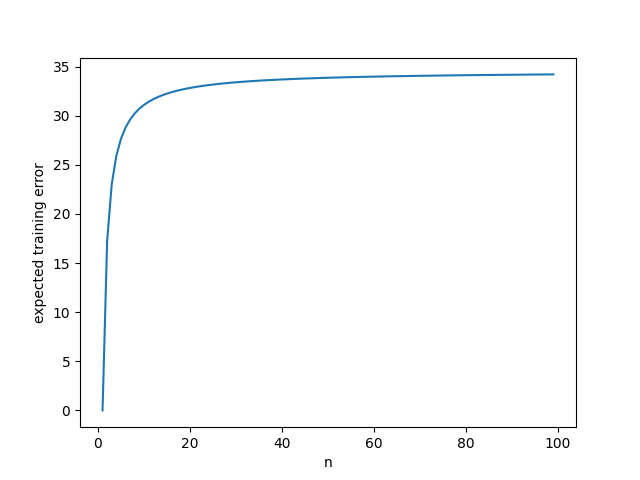
\includegraphics[width=0.9\textwidth]{training_error}}
(Note: graph shows expected error for one sample total error is value times number of training samples)

We can see that this error starts on 0 for 1 sample (as said in task c)) then increases and approach $34.56n$ which was expected error of optimal solution.
(Note: graph shows expected error for one sample total error is value times number of samples)


Now we want to compute expected testing error. We will use same approach as before we know that probability of our training sample have $i$ samples generated using first equation is $p_i=\binom{n}{i}0.4^i0.6^{n-i}$ and optimal $b_i$ in this case is $b_i = \frac{7i-5(n-i)}{n}$. In part b) we computed optimal error, if we put in that equation our new $b_i$ instead of optimal $b$, and multiply this error value by our probability of having $i$ samples generated using first equation we get contribution of this situation to total testing error (we denote it as $C_i^{(2)}$).

 \begin{align*}
 	C_i^{(2)} = \binom{n}{i}0.4^i0.6^{n-i}E_i^{(2)}(b_i)
 	\\
 	\text{(note: using equation from part b))}
 	\\
 	C_i^{(2)} = \binom{n}{i}0.4^i0.6^{n-i}\sum_{j=1}^{m}(0.4(2x^{(j)} + b_i - (2x^{(j)}+7))^2 + 0.6(2x^{(j)} + b_i - (2x^{(j)}-5))^2)
 	\\
 	C_i^{(2)} = \binom{n}{i}0.4^i0.6^{n-i}\sum_{j=1}^{m}((0.4(b_i-7))^2 + 0.6(b_i+5))^2))
 	\\
 	C_i^{(2)} = \binom{n}{i}0.4^i0.6^{n-i}m((0.4(\frac{7i-5(n-i)}{n}-7))^2 + 0.6(\frac{7i-5(n-i)}{n}+5))^2))
 \end{align*}

Total error is similarly to previous task just sum of all contributions.

\begin{align*}
	E^{test}(b) = \sum_{i=0}^{n} C_i^{(2)}
	\\
	E^{train}(b) = \sum_{i=0}^{n} \binom{n}{i}0.4^i0.6^{n-i}m((0.4(\frac{7i-5(n-i)}{n}-7))^2 + 0.6(\frac{7i-5(n-i)}{n}+5))^2))
\end{align*}

Now let's visualize this error using plot.

\centerline{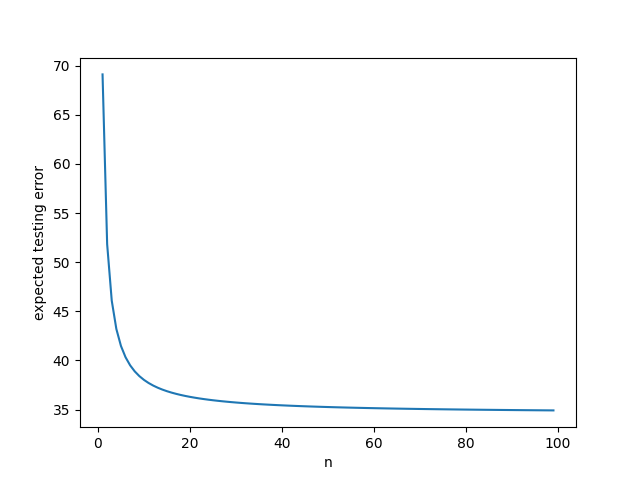
\includegraphics[width=0.9\textwidth]{testing_error}}
(Note: graph shows expected error for one sample total error is value times number of testing samples)

We can see that this error starts on $69.12$ for 1 sample (as computed in task c)) then increases and approach $34.56n$ which was expected error of optimal solution.
(Note: graph shows expected error for one sample total error is value times number of samples)

Now question is "How to set good size of training sample?". Let's do it in a way any sane engineer would do and that is to look at the plots we already have. We can see that testing error is decreasing quite significantly at first but after let's say 60 samples it's getting pretty flat so maybe 60 would not be such bad idea or few more if we want to be sure that results would be good enough.

\end{document}
